\documentclass[tikz,border=5pt]{standalone}
\usepackage{amsmath,amssymb,bm}
\usetikzlibrary{arrows.meta,fit,calc,backgrounds}

\definecolor{softblue}{RGB}{222,235,247}
\definecolor{softgreen}{RGB}{218,240,226}
\definecolor{softorange}{RGB}{253,228,206}
\definecolor{softpurple}{RGB}{235,224,246}
\definecolor{softyellow}{RGB}{255,244,204}
\definecolor{softgray}{RGB}{241,243,245}
\definecolor{ink}{RGB}{35,45,55}

\tikzset{
	flow/.style={-{Latex[length=2.3mm,width=1.5mm]},line width=0.75pt,draw=ink},
	thinflow/.style={-{Latex[length=1.8mm,width=1.2mm]},line width=0.55pt,draw=ink!85},
	small/.style={draw=ink!85,line width=0.6pt,rounded corners=2pt,align=center,
		minimum width=1.42cm,minimum height=0.78cm,inner sep=2.5pt,text=ink,
		font=\scriptsize},
	op/.style={draw=ink,line width=0.65pt,rounded corners=2pt,align=center,
		minimum width=1.72cm,minimum height=1.18cm,inner sep=3pt,text=ink,
		font=\scriptsize},
}

\begin{document}
	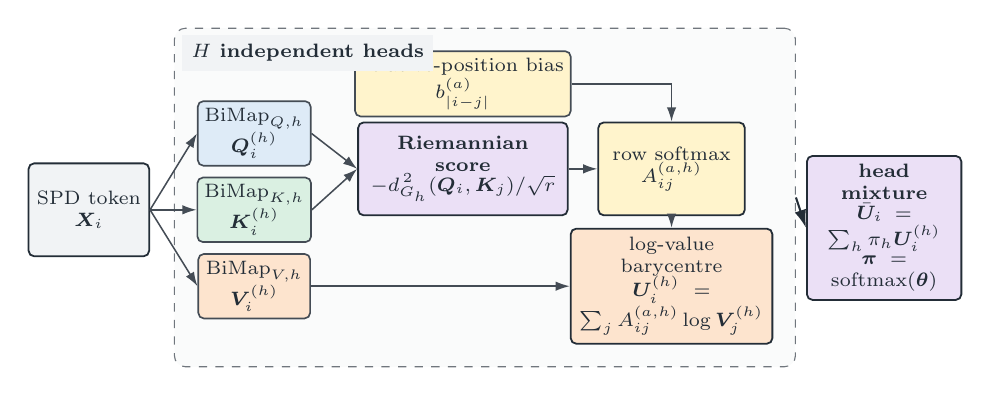
\begin{tikzpicture}[font=\sffamily]
		\node[op,fill=softgray,minimum width=1.35cm] (token) at (0.25,-2.15)
		{SPD token\\$\bm X_i$};
		\node[small,fill=softblue] (q) at (2.35,-1.18)
		{$\operatorname{BiMap}_{Q,h}$\\$\bm Q_i^{(h)}$};
		\node[small,fill=softgreen] (k) at (2.35,-2.15)
		{$\operatorname{BiMap}_{K,h}$\\$\bm K_i^{(h)}$};
		\node[small,fill=softorange] (v) at (2.35,-3.12)
		{$\operatorname{BiMap}_{V,h}$\\$\bm V_i^{(h)}$};
		\draw[thinflow] (token.east) -- (q.west);
		\draw[thinflow] (token.east) -- (k.west);
		\draw[thinflow] (token.east) -- (v.west);
		
		\node[op,fill=softpurple,text width=2.45cm] (metric) at (5.0,-1.63) {%
			\textbf{Riemannian score}\\[-1pt]
			$-d_{G_h}^{\,2}(\bm Q_i,\bm K_j)/\sqrt r$
		};
		\node[small,fill=softyellow,minimum width=2.08cm] (bias) at (5.0,-0.55) {%
			relative-position bias\\$b_{|i-j|}^{(a)}$
		};
		\node[op,fill=softyellow,text width=1.65cm] (softmax) at (7.65,-1.63) {%
			row softmax\\$A_{ij}^{(a,h)}$
		};
		\node[op,fill=softorange,text width=2.35cm] (aggregate) at (7.65,-3.12) {%
			log-value barycentre\\[-1pt]
			$\bm U_i^{(h)}=\sum_j A_{ij}^{(a,h)}\log\bm V_j^{(h)}$
		};
		\draw[thinflow] (q.east) -- (metric.west);
		\draw[thinflow] (k.east) -- (metric.west);
		\draw[thinflow] (metric.east) -- (softmax.west);
		\draw[thinflow] (bias.east) -| (softmax.north);
		\draw[thinflow] (softmax.south) -- (aggregate.north);
		\draw[thinflow] (v.east) -- (aggregate.west);
		
		\begin{scope}[on background layer]
			\node[draw=ink!65,dashed,rounded corners=4pt,fill=softgray!35,
			fit=(q)(k)(v)(metric)(bias)(softmax)(aggregate),inner sep=8pt] (headbox) {};
		\end{scope}
		\node[anchor=north west,font=\scriptsize\bfseries,text=ink,fill=softgray]
		at ($(headbox.north west)+(0.10,-0.09)$) {$H$ independent heads};
		
		\node[op,fill=softpurple,text width=1.75cm] (mix) at (10.35,-2.38) {%
			\textbf{head mixture}\\[-1pt]
			$\bar{\bm U}_i=\sum_h\pi_h\bm U_i^{(h)}$\\[-1pt]
			$\bm\pi=\operatorname{softmax}(\bm\theta)$
		};
		\draw[flow] (headbox.east) -- (mix.west);
		
		
	\end{tikzpicture}
\end{document}
